\section{Numerical Methods}\label{app:numerical}

%\monika{first revision done, please read and revise further}

%==============================================================================
\subsection{Consistency of Radiative Transfer Simulations}\label{app:radtrans}

\begin{figure*}
  \centering
  %\note{altex}
  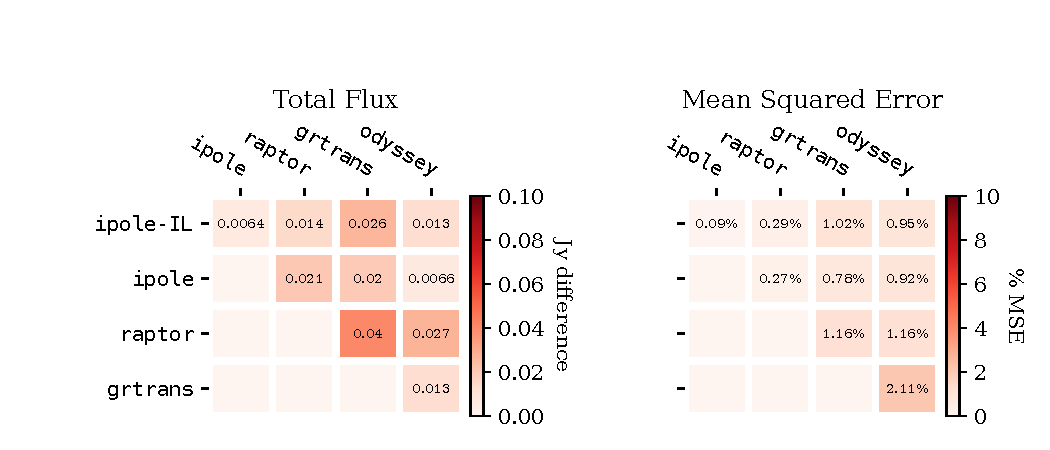
\includegraphics[width=0.95\textwidth]{figures/grmhd_hi_IntegratedUnpolarizeds_plot.pdf}
  \caption{Tables comparing the outputs from several radiative transfer codes used within the EHT for generating images of GRMHD models.  The left table compares total flux between all images (all fluxes were about 0.5\,Jy). The right table compares the Mean Squared Error, described in Section \ref{app:radtrans}, which compares image contents.}
  \label{fig:radtrans_grmhd_comp}
\end{figure*}

Two extensive studies have been undertaken within the EHT Collaboration comparing radiative transfer methods used to evaluate models.  The first, \citep{2020ApJ...897..148G}, evaluated the consistency between general relativistic ray-traced radiative transfer (GRRT) codes when tracing geodesics and when integrating the unpolarized radiative transfer equation.  The second, \citet{Prather_et_al_2022}, evaluates code performance when imaging GRMHD simulation output and when integrating the equations of polarized radiative transfer.

Several EHT radiative transfer codes participated in a comparison exercise in which each code produced an image of the same GRMHD snapshot file  with parameter chosen to realistically simulate an image of the black hole \m87 with 230\GHz total flux of 0.5\,Jy.  Figure \ref{fig:radtrans_grmhd_comp} shows tables comparing the total flux of the resulting images as well as image differences measured by the mean squared error (MSE) between images, defined as
\begin{align}
    \mathrm{MSE}(A, B) &= \frac{\sum_j|A_j-B_j|^2}{\sum_j|A_j|^2}
\end{align}
summed over each image pixel $j$. All images agree to 0.04\,Jy (8\%) in flux and to a mean squared error of 0.0211, recorded by convention as a percentage 2.11\%.  This level of agreement far exceeds the detector uncertainties in the EHT measurements of \sgra or \m87, rendering the choice of GRRT code irrelevant in producing images for analyses in this paper.

The image field of view (FOV) is another potential concern in evaluating models---the need for efficiency in generating the millions of images used in this analysis was weighed against any emission which might be missed in images with small FOV. For models that pass size and other constraints, the FOV is large enough to capture relevant emission, as shown in Figure~\ref{fig:radtrans_fov_study}.

\begin{figure}
  \centering
  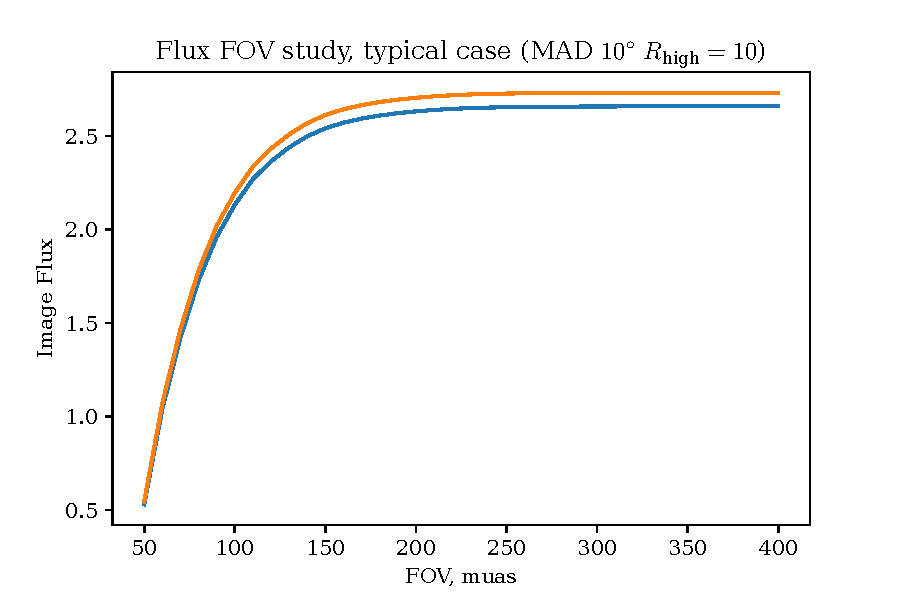
\includegraphics[width=0.45\textwidth]{figures/fov_study.pdf}
  \caption{Flux produced by an image vs the camera field of view. The nominal FOV of $200\uas$ is enough to capture 99\% of emission from this model.\monika{add what are the two different lines: what does the color codes}}
  \label{fig:radtrans_fov_study}
\end{figure}

%==============================================================================
\subsection{GRMHD Simulations Consistency and Convergence}\label{app:resolution_study}

% note: passfail tables are consistently, e.g., tab:illinoisPF or tab:VKhamrPF

%commented out cause there is only ine subsubsection here
%\subsubsection{Comparison of \kharma and \bhac thermal models}

As evident in Table~\ref{tab:GRMHDmodels} the thermal models have been calculated for an identical parameter space from two different codes, namely \kharma and \bhac for the GRMHD simulations and \ipole and \bhoss codes for the GRRT calculations. This allows us for the first time to perform an in depth comparison between the different numerical methods used in this work in addition to the EHTC code comparison projects \citep{2019ApJS..243...26P,2020ApJ...897..148G}.

\begin{figure*}
  \centering
  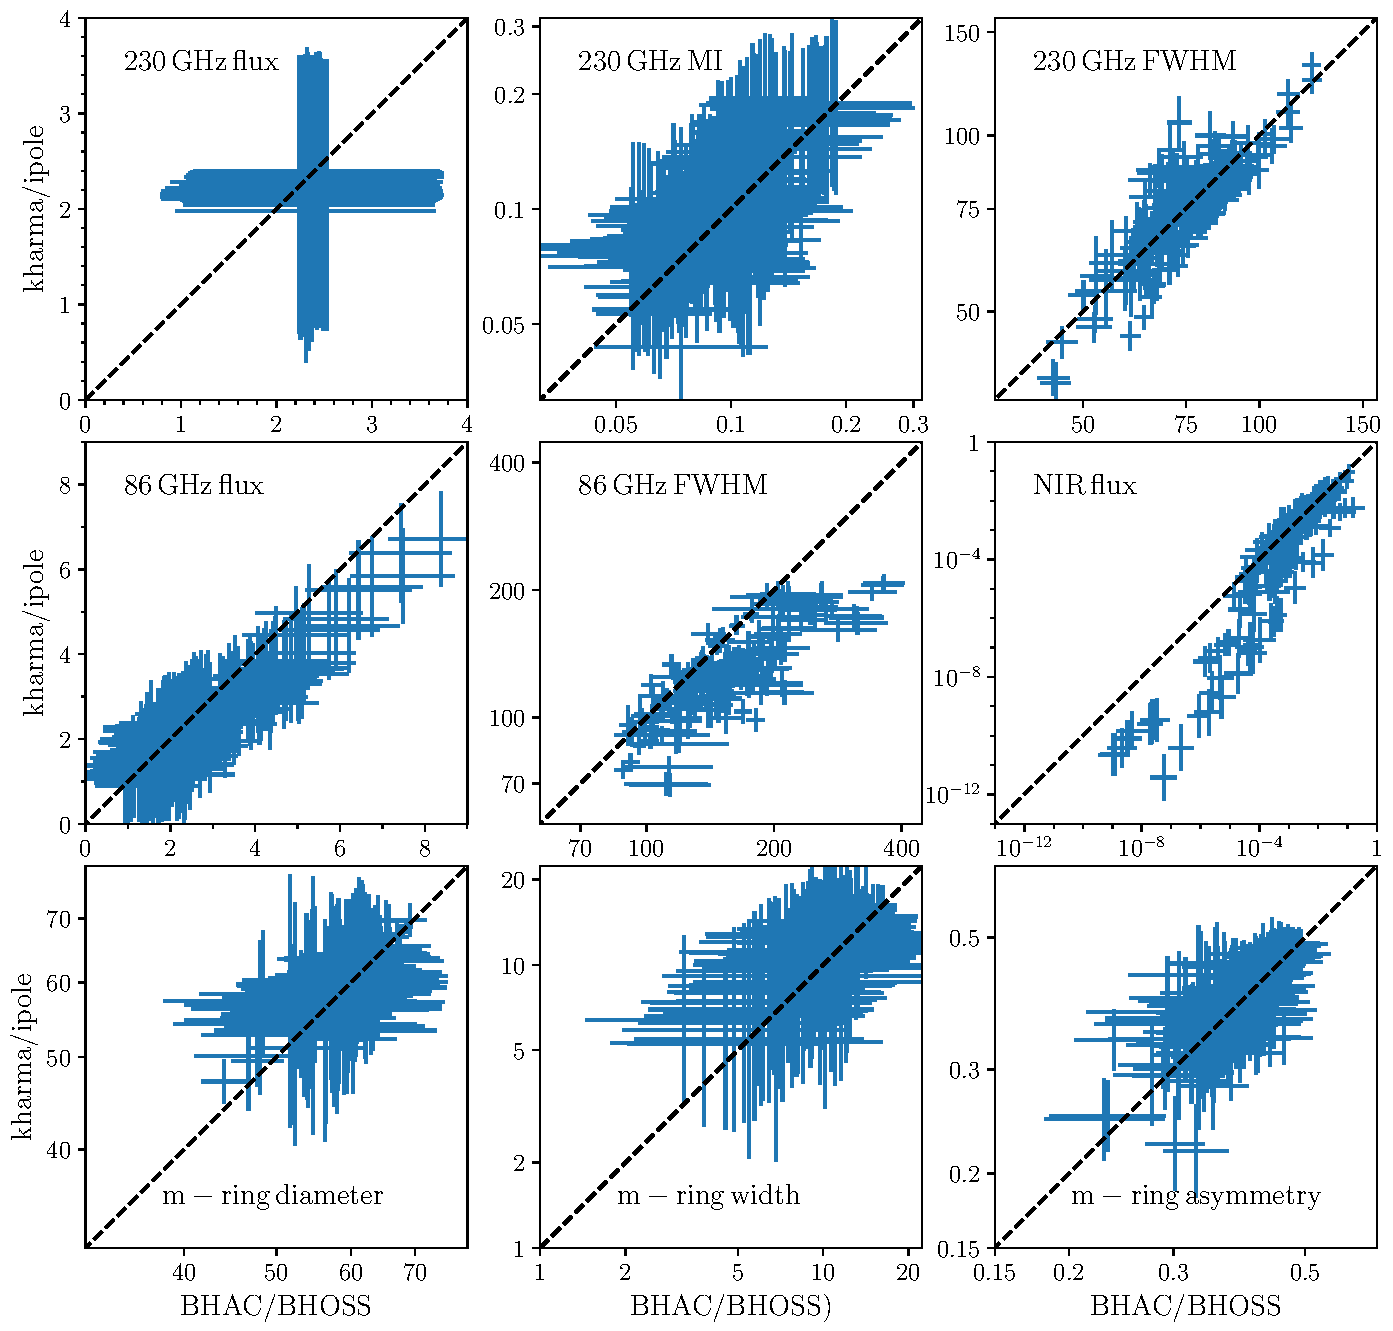
\includegraphics[width=0.8\textwidth]{./figures/BHAC_iharm_correlation2}
  \caption{Correlation between \bhac and \kharma models for 9 model constraints.  The horizontal axis is the constraint value from \bhac/\bhoss, and the vertical axis shows the constraint value from \kharma/\ipole.  Each point corresponds to a single model, with the width of the distribution shown by the error bars.  See text for details.}
  \label{fig:modelcorrelation}
\end{figure*}

In Figure \ref{fig:modelcorrelation} we show the correlation between the thermal \kharma and \bhac models for constraints where we have predictions from both models.

The top row shows from left to right the 230\,GHz flux density, the 230\GHz modulation index, MI, computed for a time window of 3 hours, and the 230\GHz image size obtained from image moments. Since we normalise the 230\GHz images to an average flux of 2.4\,Jy within a time window of 5000\,M (corresponds to 28.5 h for \sgra a mass of $4.14\times 10^6\,\msun$), the scatter around this values is small. The deviation from an ideal correlation reflects the precision and number of GRMHD snapshots included during normalization procedure.

The correlation in the 3\,hour modulation index $\mi{3}$ spreads over $\Delta \mi{3}=0.75$ which serves as a measure of intra-code ( e.g., MAD vs. SANE accretion) and inter-code (\bhac vs. \kharma) differences. Despite these differences the models show a strong correlation throughout the investigated models and parameter space.

We found a strong correlation between models and codes for the image size computed from image moments, i.e. second moments analysis.

\cfg{This may change if we recompute the major axis, etc., for the IL 86\GHz large fov images}
The middle row presents the correlation plots for the 86\GHz flux density (left), the 86\,GHz image size using second moments (middle) and the NIR flux (right). The 86\GHz flux and 86\GHz image size exhibit a shift toward larger values for the \bhac models. This difference can be explained by the larger field of view used for the \bhac models at 86\GHz during the radiative transfer calculations. Thus, more extended structure and therefore a larger total flux is included in the \bhac models. This affects mainly models with large inclinations $i\geq70^\circ$ and jet dominated emission models ($\rm{R}_{\rm high}\geq 40$).

The NIR fluxes show a tight correlation over four orders of magnitude and systematically larger flux for the \bhac models for low NIR fluxes ($\log_{10}(NIR) < -7$). These fluxes are far below the NIR constraints of $\sim 1\,\mathrm{mJy}$, and therefore they do not affect the passing or failing of the models. In the thermal models the NIR flux is generated from the tail of the electron distribution function and is thus very sensitive to the electron temperature. Small differences in the distribution and value of the electron temperature between the two codes explain the observed de-correlation at very low NIR flux.

The correlation between models for the m-ring parameters is presented in the third row of Figure~\ref{fig:modelcorrelation}. The correlation of the diameter of the m-ring is plotted in the left panel. The spread covers nearly the same extent as the 230\GHz image size (top row, right panel) however the scatter in the correlation is larger.  The same is true for the width of the m-ring (middle panel in the last row of Figure~\ref{fig:modelcorrelation}). Compared to the diameter and width of the m-ring, the asymmetry of the m-ring is less correlated (right panel). Notice that horizontal and vertical limits in the asymmetries occur since the parameter hits the boundary of the allowed range.

The smaller correlation of the m-ring parameters as compared to the other parameters presented in Figure~\ref{fig:modelcorrelation} is a consequence of the noisy nature of the m-ring fits.  Still, the distributions are quite symmetric under reflection across the diagonal, so the models are at least not biased with respect to each other.  Notice also that these plots do not capture all the information that is contained in the distribution of m-ring parameters, just the central value.

We are somewhat surprised by the strength of the correlations seen in Figure~\ref{fig:modelcorrelation}.  The range of each constraint is significantly larger than the width of the correlation, so the variations between models are real, detectable, and reproducible with independent codes.  The question of the origin of the systematic offsets between models for some constraints (for example, in the NIR) is interesting but beyond the scope of this paper.

%\monika{Dec11:  in this subsection we only show details. if hamr scoring is consistent with kharma/bhac then this should be reported in the main text, not appendix; commenting this out due to lower statistics in hamr models}

% \subsubsection{Comparison of \hamr and \kharma thermal models}

% %\note{Doosoo, Koushik to write here about HAMR thermal models.}
% Along the \kharma/\ipole and \bhac/\bhoss models, we produced a set of thermal models out to $35,000\tg$ using the GRMHD code \hamr and the GRRT code \bhoss (see Table~\ref{tab:GRMHDmodels}). These models consider a gas adiabatic index of $\Gamma_{\rm ad}=5/3$ for the SANE models and $\Gamma_{\rm ad}=13/9$ for the MAD models (Table~\ref{tab:radiativemodels}), allowing us to understand how sensitive the images are to the GRMHD fluid properties, in addition to code numerics.

% We report that overall, the \hamr/\bhoss thermal eDF images perform similarly to the \kharma/\ipole and \bhac/\bhoss models. \kc{needs verification from Michi}

% \kc{is the plan to do H-AMR and KHARMA correlations similar to figure 18?}
